\documentclass{standalone}
\usepackage{tikz}
\usetikzlibrary{patterns}
\usetikzlibrary{positioning}
\usetikzlibrary{patterns, positioning}
\usetikzlibrary{shapes.misc}
\usepackage[outline]{contour}
\contourlength{1.5pt} 
\usepackage[sfdefault]{ClearSans}

\begin{document}
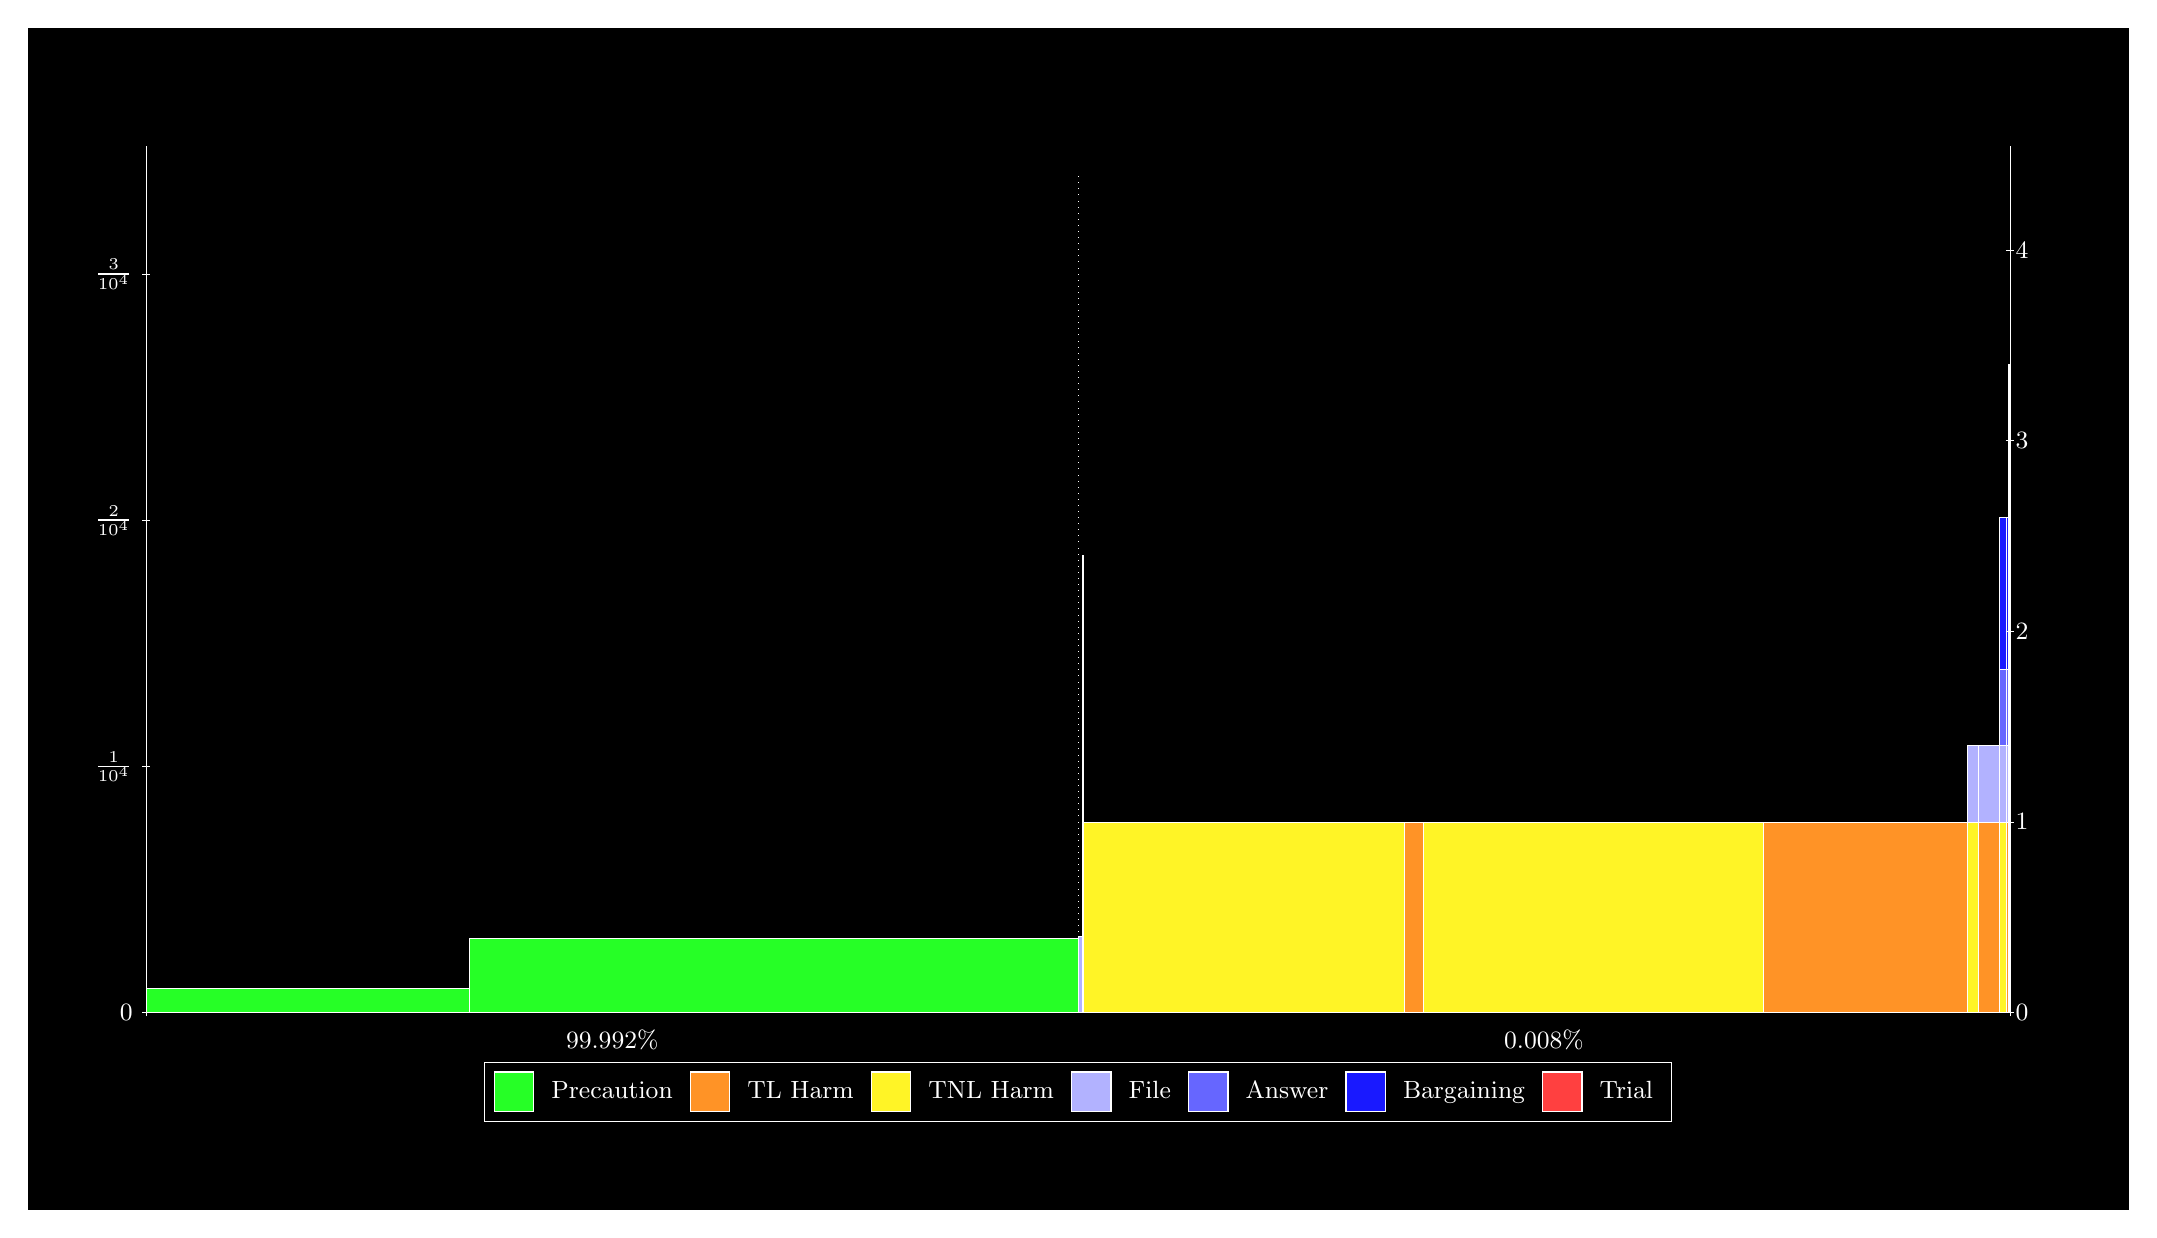
\begin{tikzpicture}
\draw[fill=black] (0,0) rectangle (26.667,15);
\draw[fill=green!85,draw=white,very thin] (1.5,2.5) rectangle (5.6005,2.8125);
\draw[fill=green!85,draw=white,very thin] (5.6005,2.5) rectangle (13.333,3.4375);
\draw[fill=green!85,draw=white,very thin] (13.333,2.5) rectangle (13.38,2.5);
\draw[fill=blue!30,draw=white,very thin] (13.333,2.5) rectangle (13.38,3.4682);
\draw[fill=green!85,draw=white,very thin] (13.38,2.5) rectangle (13.392,2.5);
\draw[fill=blue!30,draw=white,very thin] (13.38,2.5) rectangle (13.392,3.4682);
\draw[fill=blue!60,draw=white,very thin] (13.38,3.4682) rectangle (13.392,4.4364);
\draw[fill=blue!90,draw=white,very thin] (13.38,4.4364) rectangle (13.392,6.3728);
\draw[fill=green!85,draw=white,very thin] (13.392,2.5) rectangle (13.394,2.5);
\draw[fill=blue!30,draw=white,very thin] (13.392,2.5) rectangle (13.394,3.4682);
\draw[fill=blue!60,draw=white,very thin] (13.392,3.4682) rectangle (13.394,4.4364);
\draw[fill=blue!90,draw=white,very thin] (13.392,4.4364) rectangle (13.394,6.3728);
\draw[fill=red!75,draw=white,very thin] (13.392,6.3728) rectangle (13.394,8.3092);
\draw[fill=green!85,draw=white,very thin] (13.394,2.5) rectangle (17.478,2.5);
\draw[fill=yellow!85,draw=white,very thin] (13.394,2.5) rectangle (17.478,4.9205);
\draw[fill=green!85,draw=white,very thin] (17.478,2.5) rectangle (17.716,2.5);
\draw[fill=orange!85,draw=white,very thin] (17.478,2.5) rectangle (17.716,4.9205);
\draw[fill=green!85,draw=white,very thin] (17.716,2.5) rectangle (22.039,2.5001);
\draw[fill=yellow!85,draw=white,very thin] (17.716,2.5001) rectangle (22.039,4.9206);
\draw[fill=green!85,draw=white,very thin] (22.039,2.5) rectangle (24.622,2.5001);
\draw[fill=orange!85,draw=white,very thin] (22.039,2.5001) rectangle (24.622,4.9206);
\draw[fill=green!85,draw=white,very thin] (24.622,2.5) rectangle (24.765,2.5);
\draw[fill=yellow!85,draw=white,very thin] (24.622,2.5) rectangle (24.765,4.9205);
\draw[fill=blue!30,draw=white,very thin] (24.622,4.9205) rectangle (24.765,5.8887);
\draw[fill=green!85,draw=white,very thin] (24.765,2.5) rectangle (25.037,2.5);
\draw[fill=orange!85,draw=white,very thin] (24.765,2.5) rectangle (25.037,4.9205);
\draw[fill=blue!30,draw=white,very thin] (24.765,4.9205) rectangle (25.037,5.8887);
\draw[fill=green!85,draw=white,very thin] (25.037,2.5) rectangle (25.123,2.5);
\draw[fill=yellow!85,draw=white,very thin] (25.037,2.5) rectangle (25.123,4.9205);
\draw[fill=blue!30,draw=white,very thin] (25.037,4.9205) rectangle (25.123,5.8887);
\draw[fill=blue!60,draw=white,very thin] (25.037,5.8887) rectangle (25.123,6.8569);
\draw[fill=blue!90,draw=white,very thin] (25.037,6.8569) rectangle (25.123,8.7933);
\draw[fill=green!85,draw=white,very thin] (25.123,2.5) rectangle (25.146,2.5);
\draw[fill=orange!85,draw=white,very thin] (25.123,2.5) rectangle (25.146,4.9205);
\draw[fill=blue!30,draw=white,very thin] (25.123,4.9205) rectangle (25.146,5.8887);
\draw[fill=blue!60,draw=white,very thin] (25.123,5.8887) rectangle (25.146,6.8569);
\draw[fill=blue!90,draw=white,very thin] (25.123,6.8569) rectangle (25.146,8.7933);
\draw[fill=green!85,draw=white,very thin] (25.146,2.5) rectangle (25.156,2.5);
\draw[fill=yellow!85,draw=white,very thin] (25.146,2.5) rectangle (25.156,4.9205);
\draw[fill=blue!30,draw=white,very thin] (25.146,4.9205) rectangle (25.156,5.8887);
\draw[fill=blue!60,draw=white,very thin] (25.146,5.8887) rectangle (25.156,6.8569);
\draw[fill=blue!90,draw=white,very thin] (25.146,6.8569) rectangle (25.156,8.7933);
\draw[fill=red!75,draw=white,very thin] (25.146,8.7933) rectangle (25.156,10.73);
\draw[fill=green!85,draw=white,very thin] (25.156,2.5) rectangle (25.167,2.5);
\draw[fill=orange!85,draw=white,very thin] (25.156,2.5) rectangle (25.167,4.9205);
\draw[fill=blue!30,draw=white,very thin] (25.156,4.9205) rectangle (25.167,5.8887);
\draw[fill=blue!60,draw=white,very thin] (25.156,5.8887) rectangle (25.167,6.8569);
\draw[fill=blue!90,draw=white,very thin] (25.156,6.8569) rectangle (25.167,8.7933);
\draw[fill=red!75,draw=white,very thin] (25.156,8.7933) rectangle (25.167,10.73);
\draw[white,very thin] (1.5,2.5) -- (1.5,13.5);
\draw[white,very thin] (1.45,2.5) -- (1.55,2.5);
\node[font=\small,text=white, anchor=east] at (1.45, 2.5) {0};
\draw[white,very thin] (1.45,5.625) -- (1.55,5.625);
\node[font=\small,text=white, anchor=east] at (1.45, 5.625) {$\frac{1}{10^{4}}$};
\draw[white,very thin] (1.45,8.7499) -- (1.55,8.7499);
\node[font=\small,text=white, anchor=east] at (1.45, 8.7499) {$\frac{2}{10^{4}}$};
\draw[white,very thin] (1.45,11.875) -- (1.55,11.875);
\node[font=\small,text=white, anchor=east] at (1.45, 11.875) {$\frac{3}{10^{4}}$};

\draw[white,dotted,very thin] (13.333,2.83) -- (13.333,13.17);
\draw[white,very thin] (25.167,2.5) -- (25.167,13.5);
\draw[white,very thin] (25.117,2.5) -- (25.217,2.5);
\node[font=\small,text=white, anchor=west] at (25.117, 2.5) {0};
\draw[white,very thin] (25.117,4.9205) -- (25.217,4.9205);
\node[font=\small,text=white, anchor=west] at (25.117, 4.9205) {1};
\draw[white,very thin] (25.117,7.341) -- (25.217,7.341);
\node[font=\small,text=white, anchor=west] at (25.117, 7.341) {2};
\draw[white,very thin] (25.117,9.7615) -- (25.217,9.7615);
\node[font=\small,text=white, anchor=west] at (25.117, 9.7615) {3};
\draw[white,very thin] (25.117,12.182) -- (25.217,12.182);
\node[font=\small,text=white, anchor=west] at (25.117, 12.182) {4};

\draw[white,very thin] (1.5,2.5) -- (25.167,2.5);
\draw[white,very thin] (1.5,2.45) -- (1.5,2.55);
\node[font=\small,text=white, anchor=north] at (1.5, 2.45) {};
\draw[white,very thin] (25.167,2.45) -- (25.167,2.55);
\node[font=\small,text=white, anchor=north] at (25.167, 2.45) {};

\node[font=\small,text=white,anchor=south] at (7.4167, 1.9) {99.992\%};
\node[font=\small,text=white,anchor=south] at (19.25, 1.9) {0.008\%};
\draw (13.3333,2.5) node (B) {};
\begin{scope}[align=center]
\matrix[scale=0.5,draw=white,below=0.5cm of B,nodes={draw},column sep=0.1cm]{
\node[rectangle,draw,minimum width=0.5cm,minimum height=0.5cm,fill=green!85]{}; & \node[draw=none,font=\small,text=white]{Precaution}; &
\node[rectangle,draw,minimum width=0.5cm,minimum height=0.5cm,fill=orange!85]{}; & \node[draw=none,font=\small,text=white]{TL Harm}; &
\node[rectangle,draw,minimum width=0.5cm,minimum height=0.5cm,fill=yellow!85]{}; & \node[draw=none,font=\small,text=white]{TNL Harm}; &
\node[rectangle,draw,minimum width=0.5cm,minimum height=0.5cm,fill=blue!30]{}; & \node[draw=none,font=\small,text=white]{File}; &
\node[rectangle,draw,minimum width=0.5cm,minimum height=0.5cm,fill=blue!60]{}; & \node[draw=none,font=\small,text=white]{Answer}; &
\node[rectangle,draw,minimum width=0.5cm,minimum height=0.5cm,fill=blue!90]{}; & \node[draw=none,font=\small,text=white]{Bargaining}; &
\node[rectangle,draw,minimum width=0.5cm,minimum height=0.5cm,fill=red!75]{}; & \node[draw=none,font=\small,text=white]{Trial}; \\\\
};\end{scope}

\end{tikzpicture}
\end{document}